\chapter{Перевірка моделі}\label{cha:model_validation}
Майже кожну, яку ми не створювали модель, треба оцінювати на наявність помилок.
У більшості (хоча і не у всіх) застосуваннях відповідним показником якості моделі є точність прогнозування.
Іншими словами, чи будуть \textit{прогнози моделі близькими до того, що насправді відбувається}.

Існує багато метрик для підведення підсумків якості моделі, але в даній роботі буде застосована середня абсолютна помилка (також звана MAE).

Помилка передбачення суми для кожного будинку:
\[error=actual-predicted\]
Отже, якщо будинок коштував \$150 000, і ви передбачали, що він коштуватиме \$100 000, помилка становить \$50 000.
За допомогою метрики MAE ми приймаємо \textit{абсолютне значення} кожної помилки.
Це перетворює кожну помилку на додатне число.
Потім беремо середнє значення цих абсолютних помилок.
Це наш показник якості моделі.
Інакше кажучи, у середньому наші прогнози відхиляються приблизно на X.

Для розрахунку MAE нам спочатку потрібна модель.

\begin{lstlisting}[style=light, language=Python,label={lst:vectorimg},caption=Розрахунок середньої абсолютної похибки]
        from sklearn.metrics import mean_absolute_error

        predicted_home_prices = melbourne_model.predict(X)
        print(mean_absolute_error(y, predicted_home_prices))
        # 434.71594577146544
\end{lstlisting}

\section{Проблема з оцінками <<в вибірці>>}\label{sec:in_sample_problem}
Значення, яки ми щойно обчислили, можна назвати оцінкою "у вибірці".
Ми використовували єдиний "зразок" будинків як для побудови моделі, так і для її оцінки.

Модель буде вважатися точною у даних тренінгу.
Модель буде дуже неточною при використанні на практиці, оскільки натренована модель не буде розпізновати нові дані, тому як шаблон не виконується.

Практична цінність моделей полягає в прогнозуванні нових даних, ми вимірюємо ефективність даних, які не використовувались для побудови моделі.
Найпростіший спосіб зробити це - виключити деякі дані з процесу побудови моделі, а потім використовувати їх для перевірки точності моделі на даних, яких вона раніше не бачила.
Ці дані називаються \textbf{даними перевірки}.

\begin{lstlisting}[style=light, language=Python,label={lst:vectorimg},caption=The mean absolute error calculcation]
        from sklearn.model_selection import train_test_split

        # split data into training and validation data, for both features and target
        # The split is based on a random number generator. Supplying a numeric value to
        # the random_state argument guarantees we get the same split every time we
        # run this script.
        train_X, val_X, train_y, val_y = train_test_split(X, y, random_state = 0)
        # Define model
        melbourne_model = DecisionTreeRegressor()
        # Fit model
        melbourne_model.fit(train_X, train_y)

        # get predicted prices on validation data
        val_predictions = melbourne_model.predict(val_X)
        print(mean_absolute_error(val_y, val_predictions))
        # 263007.8766946417
\end{lstlisting}

\section{Переобладнанням та недооснащенням}\label{sec:underfitting_overfitting}
На практиці нерідкі випадки, коли дерево має 10 розщеплень між верхнім рівнем (усі будинки) та листом.
По мірі того, як дерево стає глибшим, набір даних нарізається на листя з меншою кількістю будинків.
Якщо дерево мало лише 1 поділ, воно ділить дані на 2 групи.
Якщо кожну групу розділити знову, ми отримаємо 4 групи будинків.
Поділ кожного з них знову створить 8 груп.
Якщо ми продовжуватимемо подвоювати кількість груп, додаючи більше розділень на кожному рівні, до того, як дійдемо до 10-го рівня, у нас буде \ (2 ^ 10 \) груп будинків.
Це 1024 листки.

Коли ми ділимо будинки на багато листків, у нас також менше будинків в кожному листку.
Листя з дуже малою кількістю будинків даватимуть прогнози, які досить близькі до фактичних значень цих будинків, але вони можуть робити дуже ненадійні прогнози щодо нових даних (оскільки кожен прогноз базується лише на кількох будинках).

Це явище, яке називається \textbf{перенавчання(overfitting)}, коли модель майже ідеально відповідає навчальним даним, але погано справляється з валідацією та іншими новими даними.
З іншого боку, якщо ми зробимо наше дерево дуже дрібним, воно не ділить будинки на унікальні групи.

У крайньому випадку, якщо дерево ділить будинки лише на 2 або 4, кожна група все ще зберігає властивість різноманітності.
Очікувані прогнози можуть бути не точними для більшості будинків, навіть у даних для тренування (і це також буде погано у валідації з тієї ж причини).
Коли модель не може вловити важливі відмінності та закономірності в даних, вона буде погано працювати з навчальними даними, що називається \textbf{переобладнаннямм (underfitting)}.

Оскільки ми дбаємо про точність нових даних, які ми оцінюємо на основі наших даних перевірки, ми хочемо знайти найкращу точку між переобладнанням та недооснащенням.
Візуально нам потрібна нижня точка (червоної) кривої перевірки (див. Малюнок 3).

\begin{figure}
    \label{fig:image3}
    \centering
    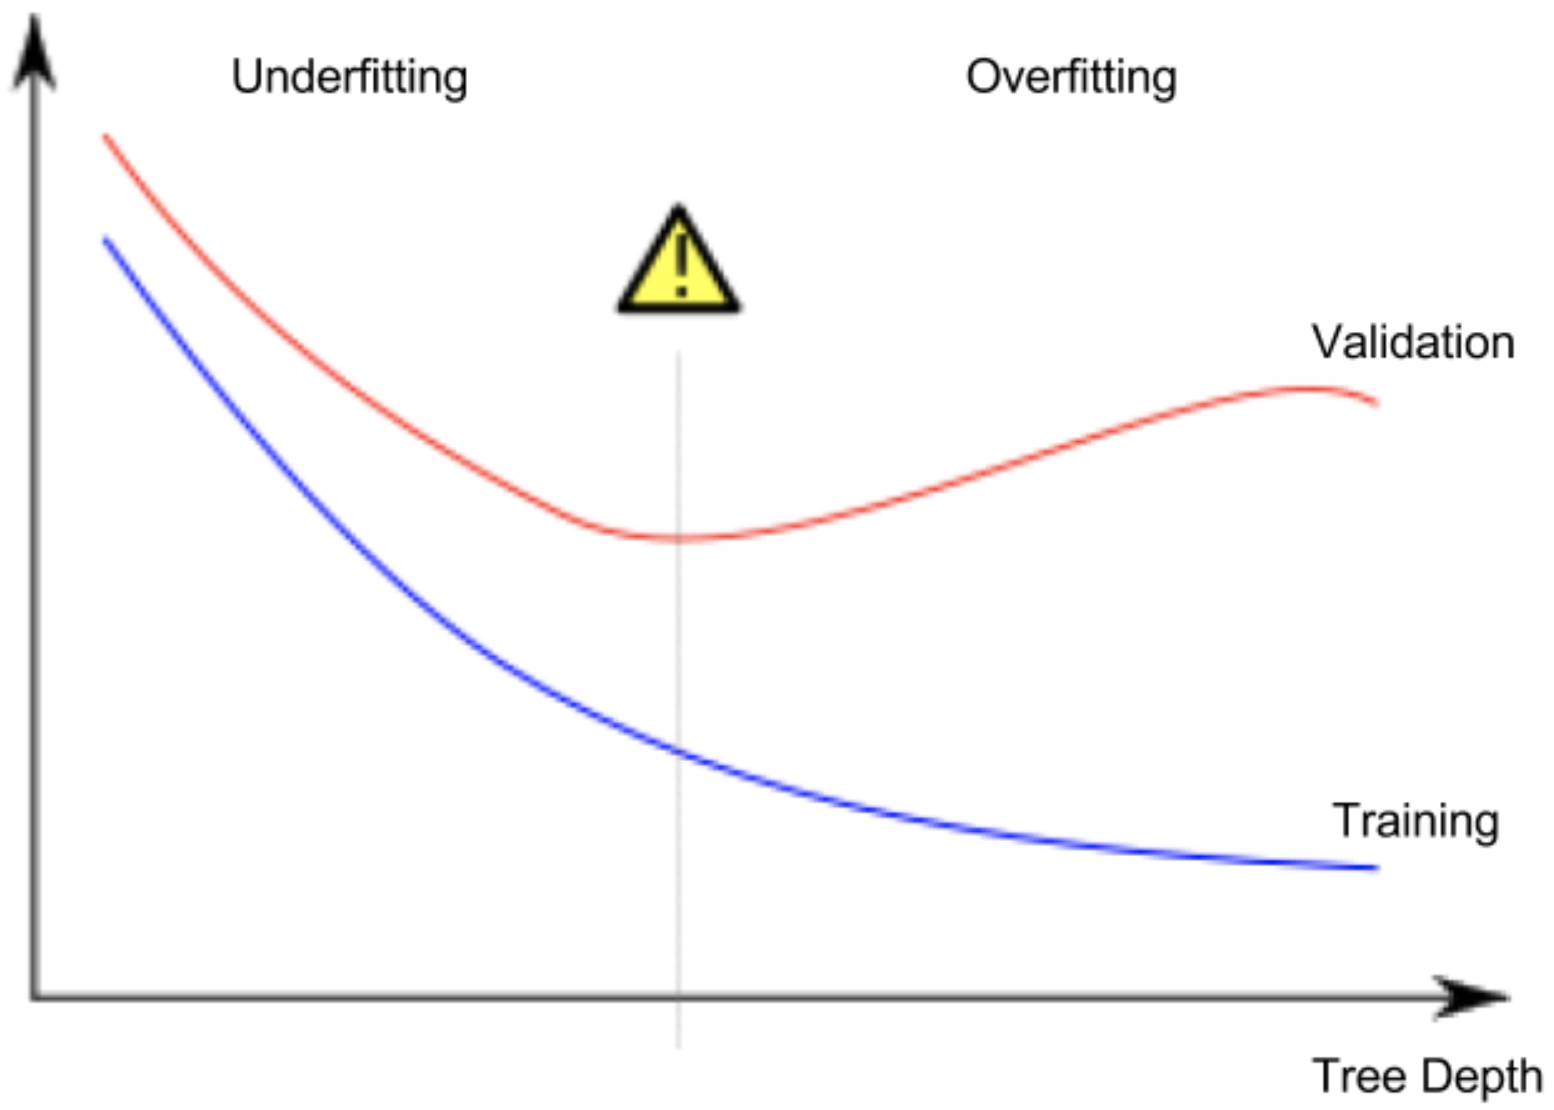
\includegraphics[scale=0.5]{image3.png}

    Deeper Trees
\end{figure}
